%% template.tex
%% from
%% bare_conf.tex
%% V1.4b
%% 2015/08/26
%% by Michael Shell
%% See:
%% http://www.michaelshell.org/
%% for current contact information.
%%
%% This is a skeleton file demonstrating the use of IEEEtran.cls
%% (requires IEEEtran.cls version 1.8b or later) with an IEEE
%% conference paper.
%%
%% Support sites:
%% http://www.michaelshell.org/tex/ieeetran/
%% http://www.ctan.org/pkg/ieeetran
%% and
%% http://www.ieee.org/

%%*************************************************************************
%% Legal Notice:
%% This code is offered as-is without any warranty either expressed or
%% implied; without even the implied warranty of MERCHANTABILITY or
%% FITNESS FOR A PARTICULAR PURPOSE!
%% User assumes all risk.
%% In no event shall the IEEE or any contributor to this code be liable for
%% any damages or losses, including, but not limited to, incidental,
%% consequential, or any other damages, resulting from the use or misuse
%% of any information contained here.
%%
%% All comments are the opinions of their respective authors and are not
%% necessarily endorsed by the IEEE.
%%
%% This work is distributed under the LaTeX Project Public License (LPPL)
%% ( http://www.latex-project.org/ ) version 1.3, and may be freely used,
%% distributed and modified. A copy of the LPPL, version 1.3, is included
%% in the base LaTeX documentation of all distributions of LaTeX released
%% 2003/12/01 or later.
%% Retain all contribution notices and credits.
%% ** Modified files should be clearly indicated as such, including  **
%% ** renaming them and changing author support contact information. **
%%*************************************************************************


% *** Authors should verify (and, if needed, correct) their LaTeX system  ***
% *** with the testflow diagnostic prior to trusting their LaTeX platform ***
% *** with production work. The IEEE's font choices and paper sizes can   ***
% *** trigger bugs that do not appear when using other class files.       ***                          ***
% The testflow support page is at:
% http://www.michaelshell.org/tex/testflow/

\documentclass[conference,final,]{IEEEtran}
% Some Computer Society conferences also require the compsoc mode option,
% but others use the standard conference format.
%
% If IEEEtran.cls has not been installed into the LaTeX system files,
% manually specify the path to it like:
% \documentclass[conference]{../sty/IEEEtran}





% Some very useful LaTeX packages include:
% (uncomment the ones you want to load)


% *** MISC UTILITY PACKAGES ***
%
%\usepackage{ifpdf}
% Heiko Oberdiek's ifpdf.sty is very useful if you need conditional
% compilation based on whether the output is pdf or dvi.
% usage:
% \ifpdf
%   % pdf code
% \else
%   % dvi code
% \fi
% The latest version of ifpdf.sty can be obtained from:
% http://www.ctan.org/pkg/ifpdf
% Also, note that IEEEtran.cls V1.7 and later provides a builtin
% \ifCLASSINFOpdf conditional that works the same way.
% When switching from latex to pdflatex and vice-versa, the compiler may
% have to be run twice to clear warning/error messages.






% *** CITATION PACKAGES ***
%
%\usepackage{cite}
% cite.sty was written by Donald Arseneau
% V1.6 and later of IEEEtran pre-defines the format of the cite.sty package
% \cite{} output to follow that of the IEEE. Loading the cite package will
% result in citation numbers being automatically sorted and properly
% "compressed/ranged". e.g., [1], [9], [2], [7], [5], [6] without using
% cite.sty will become [1], [2], [5]--[7], [9] using cite.sty. cite.sty's
% \cite will automatically add leading space, if needed. Use cite.sty's
% noadjust option (cite.sty V3.8 and later) if you want to turn this off
% such as if a citation ever needs to be enclosed in parenthesis.
% cite.sty is already installed on most LaTeX systems. Be sure and use
% version 5.0 (2009-03-20) and later if using hyperref.sty.
% The latest version can be obtained at:
% http://www.ctan.org/pkg/cite
% The documentation is contained in the cite.sty file itself.






% *** GRAPHICS RELATED PACKAGES ***
%
\ifCLASSINFOpdf
  % \usepackage[pdftex]{graphicx}
  % declare the path(s) where your graphic files are
  % \graphicspath{{../pdf/}{../jpeg/}}
  % and their extensions so you won't have to specify these with
  % every instance of \includegraphics
  % \DeclareGraphicsExtensions{.pdf,.jpeg,.png}
\else
  % or other class option (dvipsone, dvipdf, if not using dvips). graphicx
  % will default to the driver specified in the system graphics.cfg if no
  % driver is specified.
  % \usepackage[dvips]{graphicx}
  % declare the path(s) where your graphic files are
  % \graphicspath{{../eps/}}
  % and their extensions so you won't have to specify these with
  % every instance of \includegraphics
  % \DeclareGraphicsExtensions{.eps}
\fi
% graphicx was written by David Carlisle and Sebastian Rahtz. It is
% required if you want graphics, photos, etc. graphicx.sty is already
% installed on most LaTeX systems. The latest version and documentation
% can be obtained at:
% http://www.ctan.org/pkg/graphicx
% Another good source of documentation is "Using Imported Graphics in
% LaTeX2e" by Keith Reckdahl which can be found at:
% http://www.ctan.org/pkg/epslatex
%
% latex, and pdflatex in dvi mode, support graphics in encapsulated
% postscript (.eps) format. pdflatex in pdf mode supports graphics
% in .pdf, .jpeg, .png and .mps (metapost) formats. Users should ensure
% that all non-photo figures use a vector format (.eps, .pdf, .mps) and
% not a bitmapped formats (.jpeg, .png). The IEEE frowns on bitmapped formats
% which can result in "jaggedy"/blurry rendering of lines and letters as
% well as large increases in file sizes.
%
% You can find documentation about the pdfTeX application at:
% http://www.tug.org/applications/pdftex





% *** MATH PACKAGES ***
%
%\usepackage{amsmath}
% A popular package from the American Mathematical Society that provides
% many useful and powerful commands for dealing with mathematics.
%
% Note that the amsmath package sets \interdisplaylinepenalty to 10000
% thus preventing page breaks from occurring within multiline equations. Use:
%\interdisplaylinepenalty=2500
% after loading amsmath to restore such page breaks as IEEEtran.cls normally
% does. amsmath.sty is already installed on most LaTeX systems. The latest
% version and documentation can be obtained at:
% http://www.ctan.org/pkg/amsmath





% *** SPECIALIZED LIST PACKAGES ***
%
%\usepackage{algorithmic}
% algorithmic.sty was written by Peter Williams and Rogerio Brito.
% This package provides an algorithmic environment fo describing algorithms.
% You can use the algorithmic environment in-text or within a figure
% environment to provide for a floating algorithm. Do NOT use the algorithm
% floating environment provided by algorithm.sty (by the same authors) or
% algorithm2e.sty (by Christophe Fiorio) as the IEEE does not use dedicated
% algorithm float types and packages that provide these will not provide
% correct IEEE style captions. The latest version and documentation of
% algorithmic.sty can be obtained at:
% http://www.ctan.org/pkg/algorithms
% Also of interest may be the (relatively newer and more customizable)
% algorithmicx.sty package by Szasz Janos:
% http://www.ctan.org/pkg/algorithmicx




% *** ALIGNMENT PACKAGES ***
%
%\usepackage{array}
% Frank Mittelbach's and David Carlisle's array.sty patches and improves
% the standard LaTeX2e array and tabular environments to provide better
% appearance and additional user controls. As the default LaTeX2e table
% generation code is lacking to the point of almost being broken with
% respect to the quality of the end results, all users are strongly
% advised to use an enhanced (at the very least that provided by array.sty)
% set of table tools. array.sty is already installed on most systems. The
% latest version and documentation can be obtained at:
% http://www.ctan.org/pkg/array


% IEEEtran contains the IEEEeqnarray family of commands that can be used to
% generate multiline equations as well as matrices, tables, etc., of high
% quality.




% *** SUBFIGURE PACKAGES ***
%\ifCLASSOPTIONcompsoc
%  \usepackage[caption=false,font=normalsize,labelfont=sf,textfont=sf]{subfig}
%\else
%  \usepackage[caption=false,font=footnotesize]{subfig}
%\fi
% subfig.sty, written by Steven Douglas Cochran, is the modern replacement
% for subfigure.sty, the latter of which is no longer maintained and is
% incompatible with some LaTeX packages including fixltx2e. However,
% subfig.sty requires and automatically loads Axel Sommerfeldt's caption.sty
% which will override IEEEtran.cls' handling of captions and this will result
% in non-IEEE style figure/table captions. To prevent this problem, be sure
% and invoke subfig.sty's "caption=false" package option (available since
% subfig.sty version 1.3, 2005/06/28) as this is will preserve IEEEtran.cls
% handling of captions.
% Note that the Computer Society format requires a larger sans serif font
% than the serif footnote size font used in traditional IEEE formatting
% and thus the need to invoke different subfig.sty package options depending
% on whether compsoc mode has been enabled.
%
% The latest version and documentation of subfig.sty can be obtained at:
% http://www.ctan.org/pkg/subfig




% *** FLOAT PACKAGES ***
%

%\usepackage{fixltx2e}
% fixltx2e, the successor to the earlier fix2col.sty, was written by
% Frank Mittelbach and David Carlisle. This package corrects a few problems
% in the LaTeX2e kernel, the most notable of which is that in current
% LaTeX2e releases, the ordering of single and double column floats is not
% guaranteed to be preserved. Thus, an unpatched LaTeX2e can allow a
% single column figure to be placed prior to an earlier double column
% figure.
% Be aware that LaTeX2e kernels dated 2015 and later have fixltx2e.sty's
% corrections already built into the system in which case a warning will
% be issued if an attempt is made to load fixltx2e.sty as it is no longer
% needed.
% The latest version and documentation can be found at:
% http://www.ctan.org/pkg/fixltx2e


%\usepackage{stfloats}
% stfloats.sty was written by Sigitas Tolusis. This package gives LaTeX2e
% the ability to do double column floats at the bottom of the page as well
% as the top. (e.g., "\begin{figure*}[!b]" is not normally possible in
% LaTeX2e). It also provides a command:
%\fnbelowfloat
% to enable the placement of footnotes below bottom floats (the standard
% LaTeX2e kernel puts them above bottom floats). This is an invasive package
% which rewrites many portions of the LaTeX2e float routines. It may not work
% with other packages that modify the LaTeX2e float routines. The latest
% version and documentation can be obtained at:
% http://www.ctan.org/pkg/stfloats
% Do not use the stfloats baselinefloat ability as the IEEE does not allow
% \baselineskip to stretch. Authors submitting work to the IEEE should note
% that the IEEE rarely uses double column equations and that authors should try
% to avoid such use. Do not be tempted to use the cuted.sty or midfloat.sty
% packages (also by Sigitas Tolusis) as the IEEE does not format its papers in
% such ways.
% Do not attempt to use stfloats with fixltx2e as they are incompatible.
% Instead, use Morten Hogholm'a dblfloatfix which combines the features
% of both fixltx2e and stfloats:
%
% \usepackage{dblfloatfix}
% The latest version can be found at:
% http://www.ctan.org/pkg/dblfloatfix




% *** PDF, URL AND HYPERLINK PACKAGES ***
%
%\usepackage{url}
% url.sty was written by Donald Arseneau. It provides better support for
% handling and breaking URLs. url.sty is already installed on most LaTeX
% systems. The latest version and documentation can be obtained at:
% http://www.ctan.org/pkg/url
% Basically, \url{my_url_here}.




% *** Do not adjust lengths that control margins, column widths, etc. ***
% *** Do not use packages that alter fonts (such as pslatex).         ***
% There should be no need to do such things with IEEEtran.cls V1.6 and later.
% (Unless specifically asked to do so by the journal or conference you plan
% to submit to, of course. )



%% BEGIN MY ADDITIONS %%


\usepackage{graphicx}
% We will generate all images so they have a width \maxwidth. This means
% that they will get their normal width if they fit onto the page, but
% are scaled down if they would overflow the margins.
\makeatletter
\def\maxwidth{\ifdim\Gin@nat@width>\linewidth\linewidth
\else\Gin@nat@width\fi}
\makeatother
\let\Oldincludegraphics\includegraphics
\renewcommand{\includegraphics}[1]{\Oldincludegraphics[width=\maxwidth]{#1}}

\usepackage[unicode=true]{hyperref}

\hypersetup{
            pdftitle={Análisis de variables climáticas del páramo la Rusia en el municipio de Duitama, departamento de Boyacá},
            pdfkeywords={Páramo, variables climáticas, Correlación},
            pdfborder={0 0 0},
            breaklinks=true}
\urlstyle{same}  % don't use monospace font for urls

% Pandoc toggle for numbering sections (defaults to be off)
\setcounter{secnumdepth}{0}

% Pandoc syntax highlighting


% Pandoc header

\providecommand{\tightlist}{%
  \setlength{\itemsep}{0pt}\setlength{\parskip}{0pt}}

%% END MY ADDITIONS %%


\hyphenation{op-tical net-works semi-conduc-tor}

\begin{document}
%
% paper title
% Titles are generally capitalized except for words such as a, an, and, as,
% at, but, by, for, in, nor, of, on, or, the, to and up, which are usually
% not capitalized unless they are the first or last word of the title.
% Linebreaks \\ can be used within to get better formatting as desired.
% Do not put math or special symbols in the title.
\title{Análisis de variables climáticas del páramo la Rusia en el municipio de
Duitama, departamento de Boyacá}

% author names and affiliations
% use a multiple column layout for up to three different
% affiliations

\author{

%% ---- classic IEEETrans wide authors' list ----------------
 % -- end affiliation.wide
%% ----------------------------------------------------------



%% ---- classic IEEETrans one column per institution --------
 %% -- beg if/affiliation.institution-columnar
\IEEEauthorblockN{
  %% -- beg for/affiliation.institution.author
Camilo Andres Cruz Sanchez %% -- end for/affiliation.institution.author
}
\IEEEauthorblockA{Departamento de Ciencias Forestales\\
Universidad Nacional de Colombia\\
Medellín, Antioquia
\\cacruzs@unal.edu.co
}
\and
\IEEEauthorblockN{
  %% -- beg for/affiliation.institution.author
Natali Andrea Lopez Toro %% -- end for/affiliation.institution.author
}
\IEEEauthorblockA{Area Curricular de Medio Ambiente\\
Universidad Nacional de Colombia\\
Medellín, Antioquia
\\naalopezto@unal.edu.co
}
\and
\IEEEauthorblockN{
  %% -- beg for/affiliation.institution.author
Juan David Leon Torres %% -- end for/affiliation.institution.author
}
\IEEEauthorblockA{Departamento de Ciencias Forestales\\
Universidad Nacional de Colombia\\
Medellín, Antioquia
\\judleonto@unal.edu.co
}
\and
\IEEEauthorblockN{
  %% -- beg for/affiliation.institution.author
Cristian Camilo Gañan Tapasco %% -- end for/affiliation.institution.author
}
\IEEEauthorblockA{Departamento de Ciencias Forestales\\
Universidad Nacional de Colombia\\
Medellín, Antioquia
\\ccganant@unal.edu.co
}
\and
\IEEEauthorblockN{
  %% -- beg for/affiliation.institution.author
Juan José Olarte Zapata %% -- end for/affiliation.institution.author
}
\IEEEauthorblockA{Departamento de Ciencias Forestales\\
Universidad Nacional de Colombia\\
Medellín, Antioquia
\\jolartez@unal.edu.co
}
 %% -- end for/affiliation.institution
 %% -- end if/affiliation.institution-columnar
%% ----------------------------------------------------------





%% ---- one column per author, classic/default IEEETrans ----
 %% -- end if/affiliation.institution-columnar
%% ----------------------------------------------------------

}

% conference papers do not typically use \thanks and this command
% is locked out in conference mode. If really needed, such as for
% the acknowledgment of grants, issue a \IEEEoverridecommandlockouts
% after \documentclass

% for over three affiliations, or if they all won't fit within the width
% of the page, use this alternative format:
%
%\author{\IEEEauthorblockN{Michael Shell\IEEEauthorrefmark{1},
%Homer Simpson\IEEEauthorrefmark{2},
%James Kirk\IEEEauthorrefmark{3},
%Montgomery Scott\IEEEauthorrefmark{3} and
%Eldon Tyrell\IEEEauthorrefmark{4}}
%\IEEEauthorblockA{\IEEEauthorrefmark{1}School of Electrical and Computer Engineering\\
%Georgia Institute of Technology,
%Atlanta, Georgia 30332--0250\\ Email: see http://www.michaelshell.org/contact.html}
%\IEEEauthorblockA{\IEEEauthorrefmark{2}Twentieth Century Fox, Springfield, USA\\
%Email: homer@thesimpsons.com}
%\IEEEauthorblockA{\IEEEauthorrefmark{3}Starfleet Academy, San Francisco, California 96678-2391\\
%Telephone: (800) 555--1212, Fax: (888) 555--1212}
%\IEEEauthorblockA{\IEEEauthorrefmark{4}Tyrell Inc., 123 Replicant Street, Los Angeles, California 90210--4321}}




% use for special paper notices
%\IEEEspecialpapernotice{(Invited Paper)}




% make the title area
\maketitle

% As a general rule, do not put math, special symbols or citations
% in the abstract
\begin{abstract}
Los páramos son ecosistemas muy complejos e importantes por el papel que
juegan en la regulación y conservación del recurso hídrico, por lo cual
se hace necesario entender el comportamiento de las variables climáticas
que se presenta en ellos, es por esto que se realiza un estudio en el
páramo de La Rusia donde se toman datos de precipitación, humedad
relativa, temperatura, radiación solar y velocidad del viento para 6
meses del año 2019 a través de una estación climatológica que hace parte
de un complejo de estaciones climáticas que ha venido instalando el
equipo de trabajo del Dr.~Mark Mulligan de Kings College y dos sensores
HOBO con los cuales se midieron temperatura y humedad relativa a través
del páramo durante cuatro días del mes de marzo. Datos con los cuales se
hicieron relaciones entre las diferentes variables climáticas por medio
del software R los cuales mostraron correlaciones positivas para la
humedad relativa vs precipitación(0.38) y correlaciones negativas entre
la radiación vs humedad relativa(-0.81). Para los datos de los sensores
se realizó un modelo kriging ordinario de primer orden y transformación
logarítmica por medio del software Arcgis, el cual mostró una
disminución en la temperatura a medida que se aumentaba la altitud, pero
no con una relación lineal sino que era fluctuante.
\end{abstract}

% keywords
\begin{IEEEkeywords}
Páramo; variables climáticas; Correlación
\end{IEEEkeywords}

% use for special paper notices



% make the title area
\maketitle

% no keywords

% For peer review papers, you can put extra information on the cover
% page as needed:
% \ifCLASSOPTIONpeerreview
% \begin{center} \bfseries EDICS Category: 3-BBND \end{center}
% \fi
%
% For peerreview papers, this IEEEtran command inserts a page break and
% creates the second title. It will be ignored for other modes.
\IEEEpeerreviewmaketitle


\hypertarget{introducciuxf3n}{%
\section{Introducción}\label{introducciuxf3n}}

El páramo es uno de los ecosistemas más importantes para la captura de
agua, éste se encuentra presente en un \(99 \%\) en la Cordillera de los
Andes, en la Sierra Nevada de Santa Marta y Costa Rica, pero también
existen páramos en África, Indonesia y Papua Nueva Guinea
\cite{cabrera}. Es por esto que los páramos ubicados en la Cordillera de
los Andes han sido definidos como extensas zonas en la cima de la
cordilleras, entre el bosque andino y el límite inferior de las nieves
perpetuas \cite{cabrera}, haciendo privilegiados a los pocos países en
el mundo que cuentan con este tipo de ecosistema por la riqueza acuífera
que ellos representan. Para el caso de Colombia en el que se encuentra
el \(49 \%\) de los páramos del mundo, ocupando el \(1.7 \%\) del
territorio nacional con aproximadamente \(34\) páramos \cite{cabrera}.
De estos, según el Ministerio de Ambiente el departamento de Boyacá
cuenta con el \(18.7 \%\) del total nacional. El complejo de páramos
Guantiva- La Rusia está presente en \(16\) municipios de este
departamento; conteniendo así el páramo de La Rusia en el que se
centrará el presente informe con el fin de conocer y analizar las
variables climáticas que allí se presentan.

La altura a la que se puede encontrar un páramo no es igual para todos
los casos, pues el límite inferior de estos es variable según la
latitud, la vertiente, el clima global y la actividad humana. En América
se encuentran entre los \(3000\) y \(4800 \ msnm\) aproximadamente. Para
Colombia, en las cordilleras central y occidental está a \(3500 \ msnm\)
y en la oriental a \(3600 \ msnm\). La zonificación típica utilizada en
la alta montaña colombiana corresponde a bosque alto andino (\(3000\) a
\(3200 \ msnm\)), páramo bajo o subpáramo (entre \(3200\) y \(3500\) o
\(3600 \ msnm\)), páramo propiamente dicho (entre \(3500\) o \(3600\) y
\(4100 \ msnm\)) y superpáramo (entre \(4100\) y \(4500 \ msnm\))
\cite{ortizparamos}. Diferentes autores confirman que el clima en los
páramos realmente es muy variado, aunque se presenten condiciones de
altura similares y de proximidad \cite{paramos}. Esta variabilidad se
presenta en todas las características climáticas, tales como
precipitación, temperatura, radiación, velocidad del viento y humedad
relativa y aunque hay todavía pocas estaciones climáticas en todos los
páramos, es evidente la variación en los resultados de la medición de
estos parámetros climáticos.

Por lo general en la transición de bosque y el subpáramo las
temperaturas medias multianuales en algunos casos pueden ser incluso
menores a \(9^{\circ}C\), aproximadamente por encima de los
\(3300 \ msnm\), en el páramo medio podrían llegar a ser menores de
\(6^{\circ}C\) y ya en el superpáramo cerca de las nieves perpetuas son
inferiores a \(3^{\circ}C\) \cite{morales2019atlas}. En cuanto a la
variación de la temperatura media mensual no hay grandes cambios, sin
embargo en los páramos la temperatura puede variar a gran escala durante
el día y la noche. En la precipitación hay una amplio rango y un gran
contraste entre los páramos de Colombia, ésta puede variar entre los
\(700\) y \(5000 \ mm\) al año. Algunos de los páramos tienen un régimen
de lluvias monomodal como el páramo de Chingaza \cite{morales2019atlas}
y otros bimodal como el complejo Guantiva - La Rusia
\cite{morales2019atlas}; los páramos más húmedos se encuentran en las
vertientes oriental de la cordillera oriental y occidental de la
cordillera occidental, en cuanto a los más secos se encuentran en
ciertas áreas al interior de la cordillera oriental
\cite{morales2019atlas}. Los ecosistemas de páramo presentan una humedad
relativa alta que es variable y estacional, siendo máxima en tiempos de
lluvia y mínima en tiempos secos, usualmente en un rango que comprende
entre un \(80\) y \(90 \%\) esto debido a un factor de suma importancia
en los páramos como lo es el fenómeno de niebla \cite{morales2019atlas}.
Comúnmente la evapotranspiración en los páramos es baja pues casi
siempre el ambiente es muy cercano a la saturación y se presenta un alta
radiación ultravioleta sobre todo en periodos secos y abundancia de luz
difusa \cite{morales2019atlas}. Por último los vientos en los páramos
son muy variables pero regularmente los más intensos se dan en los
páramos que se encuentran en las vertientes de los valles interandinos
\cite{morales2019atlas}.

\hypertarget{materiales-y-muxe9todos}{%
\section{MATERIALES Y MÉTODOS}\label{materiales-y-muxe9todos}}

\hypertarget{localizaciuxf3n-y-descripciuxf3n-del-uxe1rea-de-estudio}{%
\subsection{Localización y descripción del área de
estudio}\label{localizaciuxf3n-y-descripciuxf3n-del-uxe1rea-de-estudio}}

El páramo La Rusia se encuentra ubicado en límites de los departamentos
de Boyacá y Santander, en el flanco occidental de la cordillera
oriental, entre los \(3100\) y \(4280 \ msnm\). Este páramo hace parte
de un extenso corredor de páramos y bosques alto andinos denominado como
Guantiva - La Rusia, complejo que incluye a los páramos de Cruz
Colorada, Guina, Pan de Azúcar, Carnicerías y Guata y que tiene una
extensión en área de \(119.009 \ ha\) (Corpoboyacá y CAS, 2017). En el
páramo La Rusia predomina una topografía abrupta que varía de acuerdo
con la alternancia de las formaciones geológicas presentes. El páramo
está influenciado a escala global, por la Zona de Convergencia
Intertropical (ZCIT), de la misma forma que otros páramos y de manera
local por el movimiento de las corrientes de vientos producto del
relieve, lo que genera un régimen húmedo en mayor o menor medida. El
régimen de lluvias es bimodal, con una precipitación máxima entre abril-
mayo y octubre- noviembre (UPTC, 2015).

El sitio de estudio se encuentra dentro del páramo La Rusia en la vereda
San Alejo, municipio de Duitama Boyacá; contiguo por el norte a los
límites con el municipio de Charalá departamento de Santander. El sitio
de interés para el estudio y muestreo de datos climáticos está
representado por las coordenadas \(5^{\circ}57’48.0"N\)
\(73^{\circ}05'16.3"W\) y presenta una altitud de unos \(3500\ msnm\).

\begin{figure}
\centering
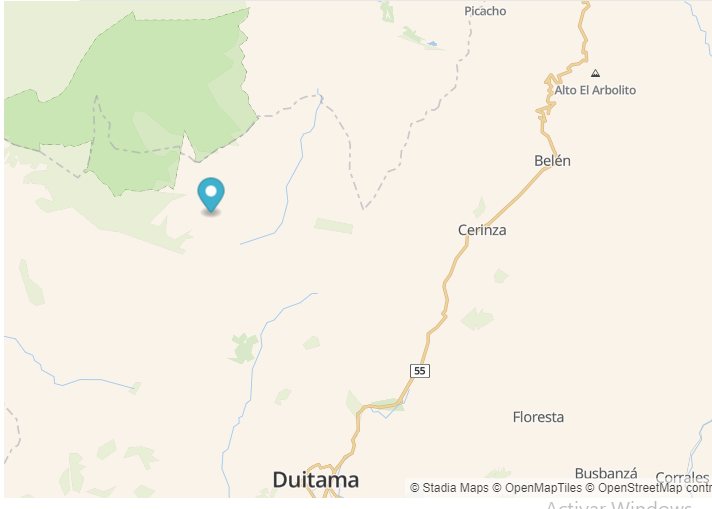
\includegraphics{mapaloc.png}
\caption{Modelo de temperatura}
\end{figure}

\hypertarget{levantamiento-de-informaciuxf3n}{%
\subsection{Levantamiento de
información}\label{levantamiento-de-informaciuxf3n}}

En una visita de varios días (13,14 y15 de marzo) al complejo de páramos
Guantiva-La rusia para el departamento de Boyacá, se instalaron varias
estaciones climáticas de tipo \texttt{Davis} con sensores para algunas
variables climáticas, que en el presente y con fines investigativos
están tomando datos climáticos(de temperatura, humedad relativa,
velocidad y dirección del viento, precipitación y radiación solar). Para
el desarrollo del análisis que se presenta en este artículo sólo se tuvo
en cuenta una estación climática de hardware y software
\texttt{Open\ source} con datos para 6 meses del año 2019, de enero a
junio; tomados cada 15 minutos para todas las variables mencionadas. La
estación climática ubicada en una cuenca del páramo, de la cual se
obtuvieron los datos, hace parte de un complejo de estaciones climáticas
instaladas por el equipo de trabajo del Dr.~Mark Mulligan de King´s
College en London, como parte de un proyecto para mejorar y calibrar
equipos de monitoreo open source más rentables para los proyectos de
tipo científico e investigativos.

También se usaron dos sensores HOBO móviles para recolectar información
de temperatura y humedad relativa en tiempo real con intervalos de
tiempo de 1 minuto por medición, los cuales fueron puestos en
funcionamiento a partir de las 8:00 hrs hasta las 17:00 hrs los días
viernes 13 de marzo y sábado 14 de marzo, y para el día domingo 15 de
marzo fueron puestos en funcionamiento entre las 8:00 hrs y las 15:00
hrs, llevando los sensores por parte del complejo de páramos Guantiva-
La Rusia, a la vez que se instalaron las estaciones climáticas y se
tomaron otros datos como caudal, calidad del agua, y muestras de suelos
con el resto del grupo de trabajo, datos que no se tendrán en cuenta
para este informe. Asimismo, se hizo uso del software de la misma
empresa (HOBO) para dispositivos celulares en el cual es posible
verificar los datos en tiempo real de las variables humedad relativa y
temperatura, y además tener estos a disposición para bajarlos en
distintos formatos de trabajo.

\hypertarget{procesamiento-de-los-datos-recolectados}{%
\subsection{Procesamiento de los datos
recolectados}\label{procesamiento-de-los-datos-recolectados}}

Los datos climáticos pueden proporcionar una gran cantidad de
información sobre el medio ambiente atmosférico que afecta a casi todos
los aspectos del esfuerzo humano \cite{Bala}, es por ello que es
importante el análisis de éstos, para determinar tendencias en las
variables que se puedan interpretar buscando entender el comportamiento
y así tomar decisiones que más convengan. Buscando el filtrado y
análisis de los datos se utilizó \texttt{R\ versión\ 3.6.1}. Para los
datos de precipitación se usó la suma de los valores diarios por mes y
para las demás (temperatura, humedad relativa y velocidad del viento)
los valores promedio. Se graficaron las variables por separado buscando
propensiones para la descripción de cada una de ellas, luego se buscaron
relaciones estadísticas entre variables con el fin de determinar acaso
alguna dependencia entre los datos. Con los datos de temperatura del
sensor HOBO se realizó un modelo Kriging ordinario de primer orden y
transformación logarítmica en el software
\texttt{ArcGIS\ versión\ 10.5}, esto con el fin de observar un
comportamiento aproximado de la variable.

\hypertarget{resultados-y-discusiuxf3n}{%
\section{Resultados y discusión}\label{resultados-y-discusiuxf3n}}

En la \textbf{Fig. 2} se puede observar la precipitación mensual
discriminada por la cantidad de precipitación de cada día (representados
en colores), en esta escala no se percibe todo el ciclo anual pero sí la
temporada de lluvias entre marzo, mayo y parte de una temporada seca a
la que se debe la baja precipitación en febrero, lo que responde al
régimen bimodal del páramo La Rusia. La precipitación total de estos 6
meses suma \(1096.2mm\), una precipitación alta, característica de las
laderas orientadas al occidente, pues las laderas internas de los Andes
están altamente influenciadas por efectos de sombra y lluvia, para las
lluvias que llegan tanto desde la cuenca del Amazonas como de la costa
del Pacífico \cite{buytaert2006hidrologia,}.

\begin{figure}
\centering
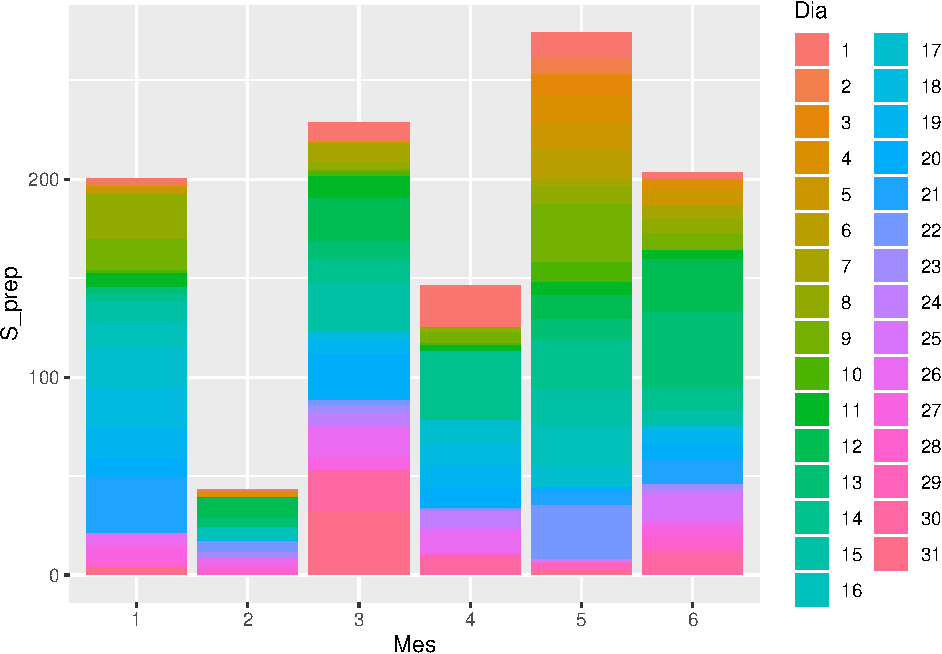
\includegraphics{Hidrology_files/figure-latex/unnamed-chunk-1-1.pdf}
\caption{Tendencia Diaría de precipitación}
\end{figure}

En la \textbf{Fig.3}, se observa la variación de la temperatura
alrededor del promedio de los seis meses de \(9.2^{\circ}C\) con una
temperatura máxima de \(19.5^{\circ}C\) y una mínima de
\(1.6^{\circ}C\), sin embargo la fluctuación de mayor densidad se
encuentra entre los \(8^{\circ}C\) y \(10^{\circ}C\). La variación
diurna de la temperatura resulta del ciclo de insolación superficial
\cite{poveda2004hidroclimatologia,}, la cual es mayor entre las 11:00
a.m. y la 1:00 p.m. Debido a su localización cercana a la línea
ecuatorial, la radiación solar diaria es casi constante todo el año,
esta constancia resulta en una baja variabilidad estacional en
temperatura media del aire, en contraste con el ciclo diario, el cual es
totalmente marcado \cite{buytaert2006hidrologia,}. En la \textbf{Fig.4}
se muestra la distribución de la temperatura a lo largo del periodo de
medición. Es notable un comportamiento de los datos aproximadamente
normal. De esto es posible deducir que los valores tienden a un valor
medio, es decir, que generalmente los valores de temperatura estarán en
el rango de \(9 a 10^{\circ}C\), sin embargo hay ocasiones como en el
mes 1 en donde la variable tiende a un valor más bajo de temperatura.

\begin{figure}
\centering
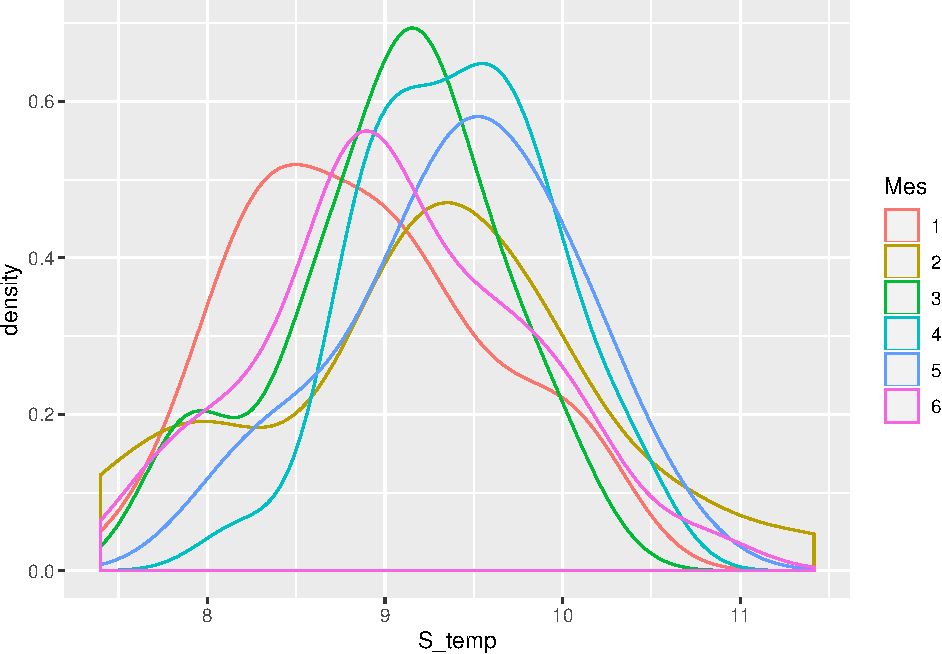
\includegraphics{Hidrology_files/figure-latex/unnamed-chunk-5-1.pdf}
\caption{Distribución de la temperatura}
\end{figure}

\begin{figure}
\centering
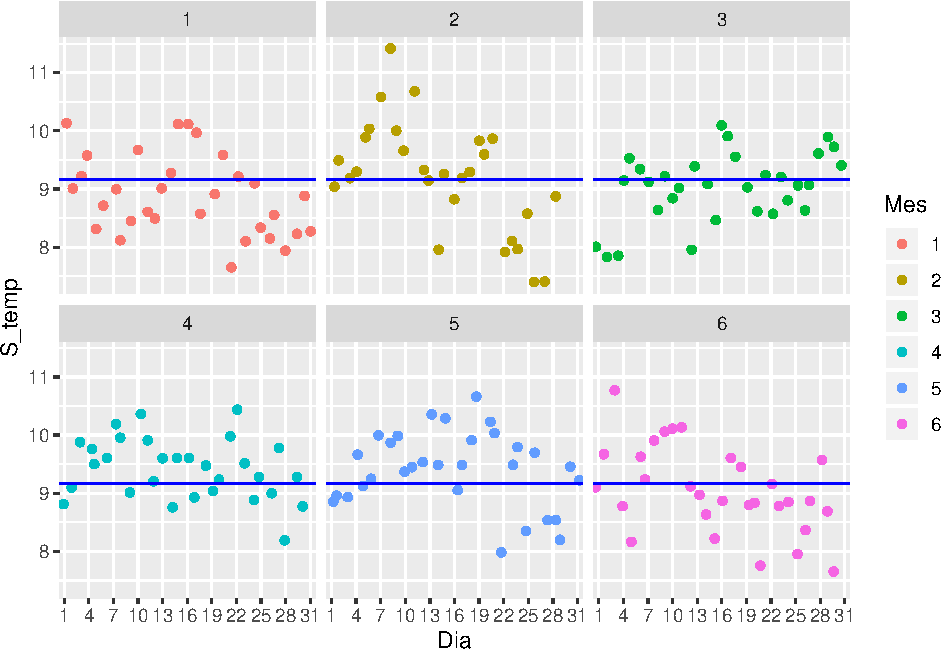
\includegraphics{Hidrology_files/figure-latex/unnamed-chunk-6-1.pdf}
\caption{Tendencia de la temperatura mensual}
\end{figure}

En la \textbf{Fig.5} se presenta la distribución de la humedad relativa;
ésta es parecida a una gráfica \texttt{Fisher}, sin embargo no tiene
relación con el caso pues no se está comparando poblaciońes, más bien
parece haber la tendencia a que en el páramo haya una alta humedad
relativa centrada en valores \(> \ 90 \%\) lo cual es relacionable con
la variable anterior pues se sabe que a mayor temperatura del aire hay
mayor capacidad en retener humedad \cite{jaramillo}. Se puede inferir
entonces que la temperatura del páramo es fría solo con mirar su humedad
relativa. Éste comportamiento está presente en los datos pues hay un
valor bajo de temperatura con un alto porcentaje de humedad.

\begin{figure}
\centering
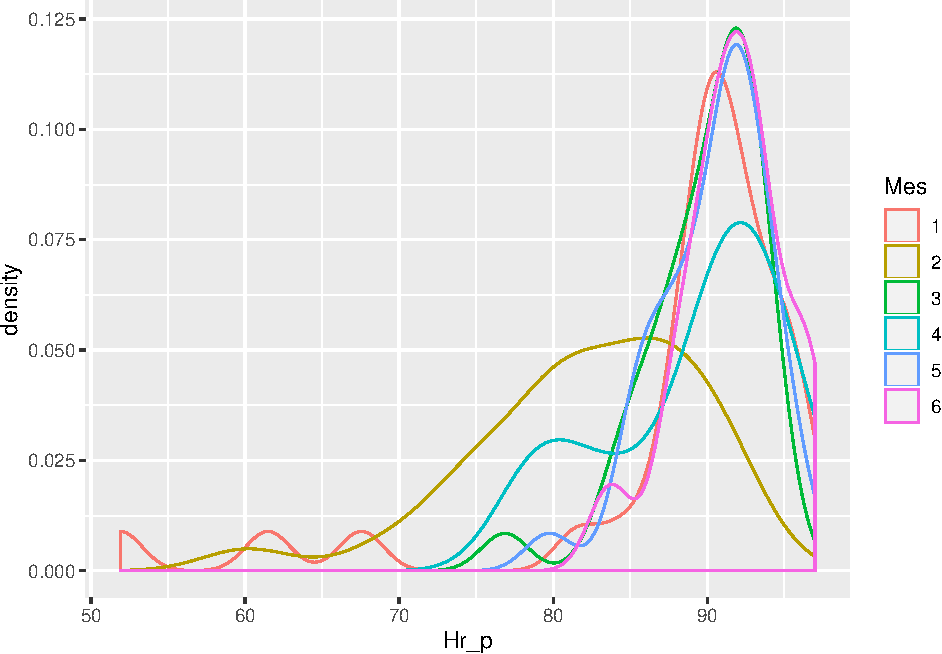
\includegraphics{Hidrology_files/figure-latex/unnamed-chunk-8-1.pdf}
\caption{Distribución de la Humedad relativa}
\end{figure}

\begin{figure}
\centering
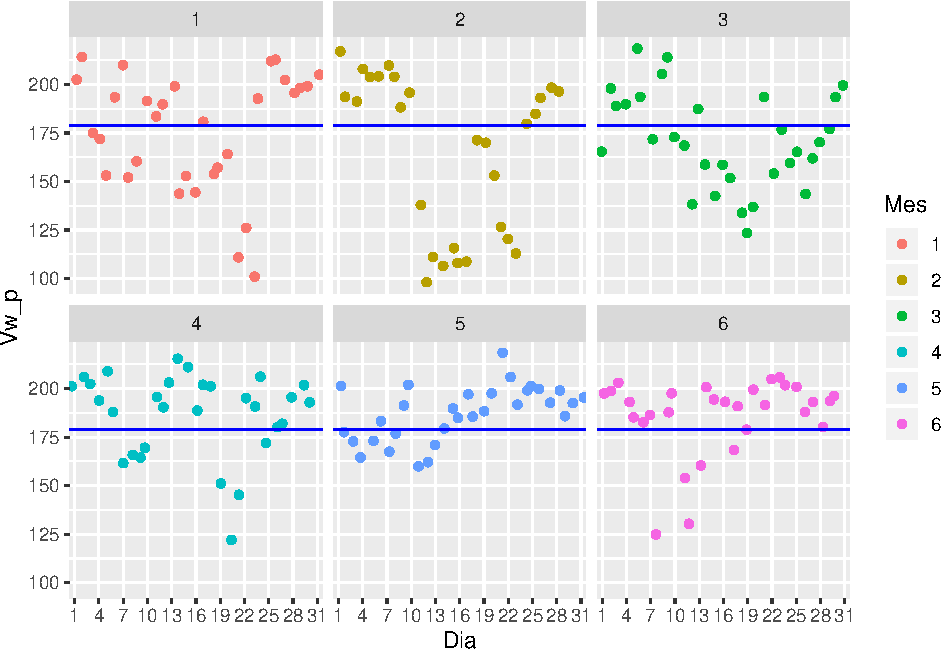
\includegraphics{Hidrology_files/figure-latex/unnamed-chunk-11-1.pdf}
\caption{Distribución de la velocidad del viento}
\end{figure}

En la \textbf{Fig.6} se muestra la distribución de los datos para la
velocidad del viento y se extrae que los valores medios oscilan entre
\(50\) y \(100 \frac{m}{s}\). Éste parámetro es relacionado con la
precipitación pues si hay fuertes vientos, éstos pueden desplazar las
masas de aire húmedas disminuyendo la probabilidad del evento
\cite{tobon}. Por ejemplo, para el mes 2 que fue el que tuvo menor
precipitación, la velocidad del viento para esa fecha es variable, lo
cual no explicaría la baja precipitación en ese mes; sin embargo, al
mirar la \textbf{Fig.7} , la distribución de la radiación solar, se
puede ver cómo en la fecha, la incidencia de los rayos solares no fue
constante lo que favoreció a su vez que la humedad relativa presentara
los valores más pequeños en todo el registro. Las masas de aire entonces
se calientan cuando hay una temperatura mayor debido a más radiación
solar, éstas ascienden y la velocidad del viento puede o no llevarlas a
otro lugar controlando así la precipitación en el sitio \cite{tobon}.

\begin{figure}
\centering
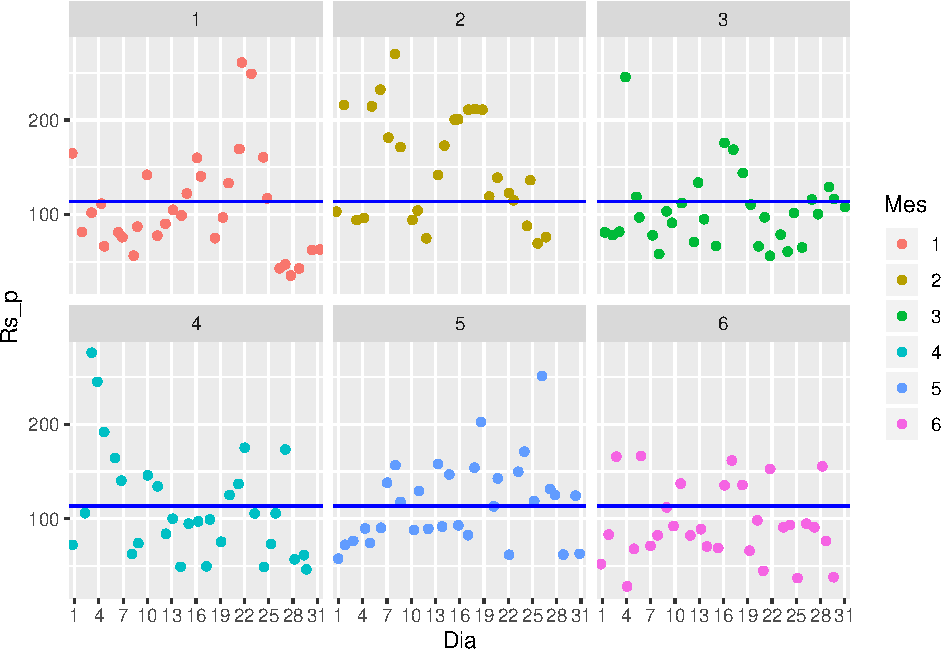
\includegraphics{Hidrology_files/figure-latex/unnamed-chunk-14-1.pdf}
\caption{Distribución de la radiación solar media}
\end{figure}

En la \textbf{Fig.8} se puede observar la correlación para las distintas
variables climáticas. Se encuentra una correlación positiva entre la
precipitación y humedad relativa (\(0.38\)), esto puede darse ya que en
épocas de lluvia la humedad relativa es constantemente alta y tiende a
la saturación en los eventos de precipitación, además suele presentarse
el fenómeno de niebla \cite{morales2019atlas}. Relación que se puede
corroborar en la \textbf{Fig.11} que muestra la relación entre
precipitación y humedad relativa, que presenta una línea de tendencia
con un aumento muy rápido en la humedad relativa mientras inicia la
precipitación y luego se mantiene constante en el evento de lluvia
tendiendo a la saturación del ambiente. Lo mismo ocurre con las
variables de radiación solar y temperatura que tienen una correlación
positiva de \(0.52\), la cual puede ser el resultado del gran aumento de
insolación solar y temperatura que se presenta a medio día en el páramo
ya que se encuentra muy cerca de la línea ecuatorial y recibe una gran
radiación diaria todo el año mientras se tenga un cielo despejado
\cite{buytaert2006hidrologia}. Esto se puede ver en la \textbf{Fig.10}
que muestra la relación entre temperatura y radiación solar, donde la
línea de tendencia muestra una relación directa en el aumento de la
radiación y temperatura. Es el caso contrario cuando se analiza la
correlación entre radiación solar y humedad relativa (\(-0.81\)) o
temperatura y humedad relativa (\(-0.25\)), obteniendo valores
negativos; esto se pudo evidenciar en campo, pues mientras la
temperatura era más alta el aire se sentía mucho más seco, como se puede
ver en la \textbf{Fig.9} que muestra la relación entre temperatura vs
humedad relativa, donde la línea de tendencia disminuye a medida que la
temperatura aumenta. La gráfica de dispersión ilustra un comportamiento
inverso entre las dos variables con una línea de tendencia que en
general es decreciente, a medida que comienza a ascender la temperatura
la humedad relativa comienza a descender, lo que es normal pues a medida
que el ambiente se torna más caliente, este se tornara más seco lo que
en un páramo está sujeto a la estacionalidad, pues la humedad relativa
es variable y estacional \cite{hofstede2017p}, así en épocas de lluvia
habrá mayor humedad relativa que en épocas secas o de verano, la
variación de este factor está estrechamente ligada a los fenómenos de
niebla que en un páramo pueden presentarse con mayor o menor frecuencia
dentro de un periodo de tiempo. En síntesis la gráfica no se sale del
comportamiento general de estos dos parámetros climáticos (humedad
relativa y temperatura), debido a que éstos son normalmente inversos.
Cabe destacar que la humedad relativa extrañamente baja a valores
menores de \(70 \%\) lo que es característico de estos ecosistemas.
\cite{hofstede2017p}

\begin{figure}
\centering
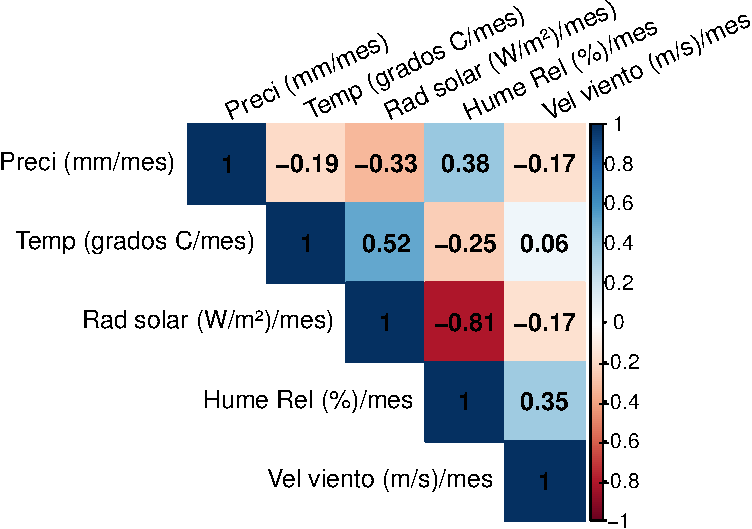
\includegraphics{Hidrology_files/figure-latex/unnamed-chunk-18-1.pdf}
\caption{Matrix de correlación para las variables climáticas}
\end{figure}

\begin{figure}
\centering
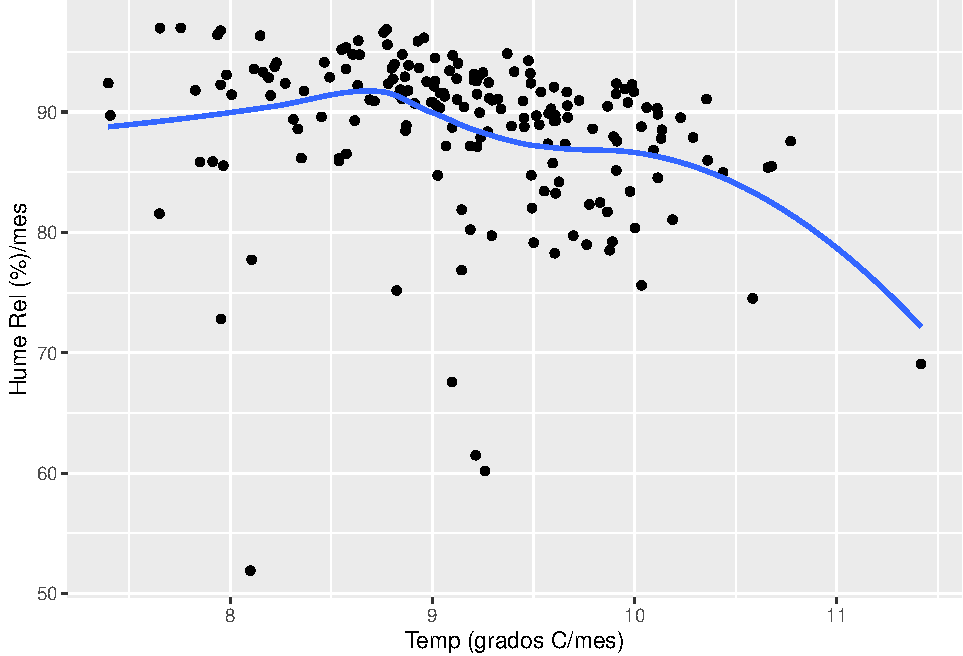
\includegraphics{Hidrology_files/figure-latex/unnamed-chunk-19-1.pdf}
\caption{Temperatura vs Humedad relativa}
\end{figure}

\begin{figure}
\centering
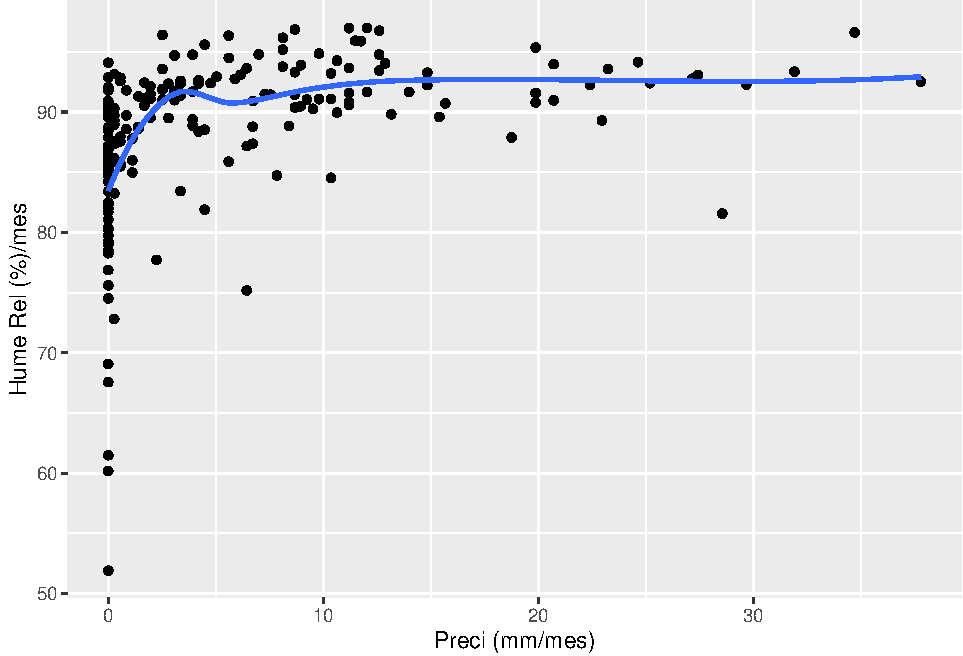
\includegraphics{Hidrology_files/figure-latex/unnamed-chunk-20-1.pdf}
\caption{Temperatura vs Radiación solar}
\end{figure}

\begin{figure}
\centering
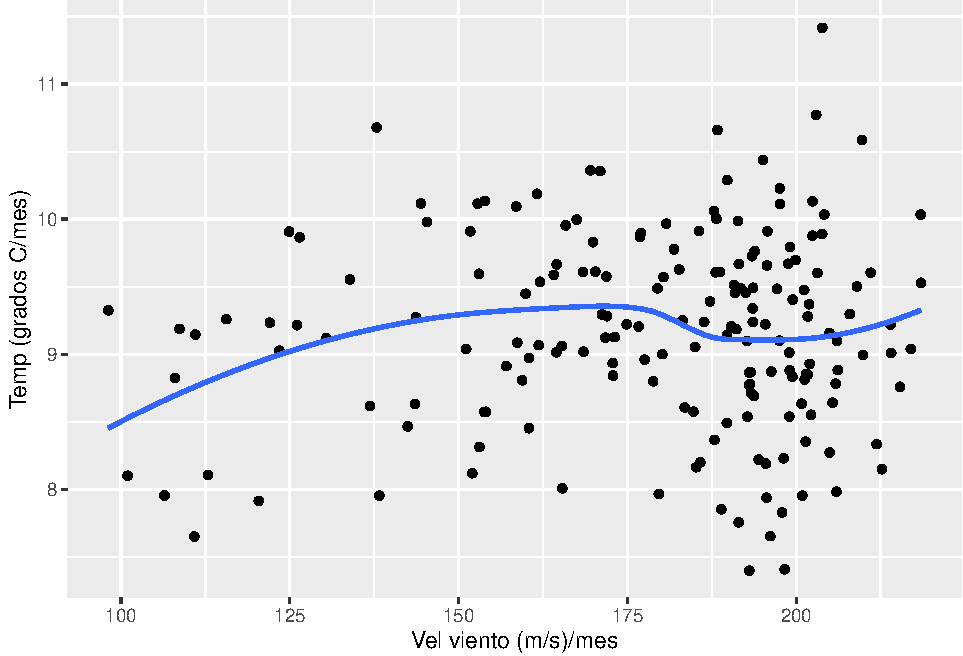
\includegraphics{Hidrology_files/figure-latex/unnamed-chunk-21-1.pdf}
\caption{Precipitación vs Humedad relativa}
\end{figure}

\begin{figure}
\centering
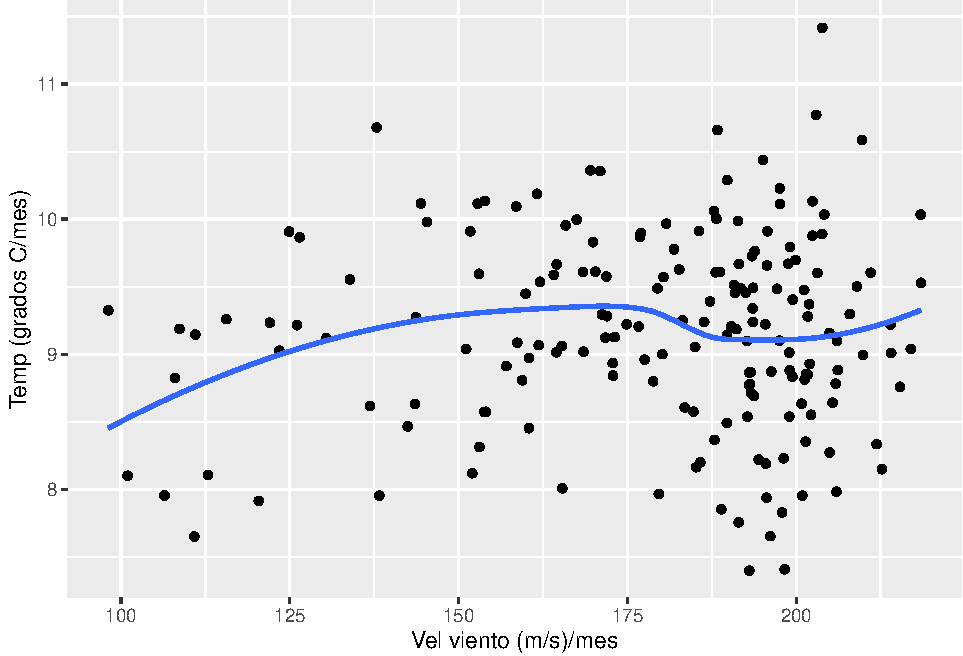
\includegraphics{Hidrology_files/figure-latex/unnamed-chunk-22-1.pdf}
\caption{Velocidad del viento vs Temperatura}
\end{figure}

En la \textbf{Fig.10} se observa la relación entre la temperatura y la
radiación solar para el páramo La Rusia, de la gráfica se deduce que
estos dos parámetros son directamente proporcionales pues en la mayoría
del tiempo a medida que la temperatura aumenta la radiación solar
comienza también a aumentar, y es que esto mientras se tengan las
condiciones necesarias (como un cielo despejado) es normal en un páramo
pues debido a su altitud y cercanía con el ecuador la radiación solar
que reciben estos ecosistemas es alta mientras no haya nubosidad
\cite{montenegro2015estimacion}.

\begin{figure}
\centering
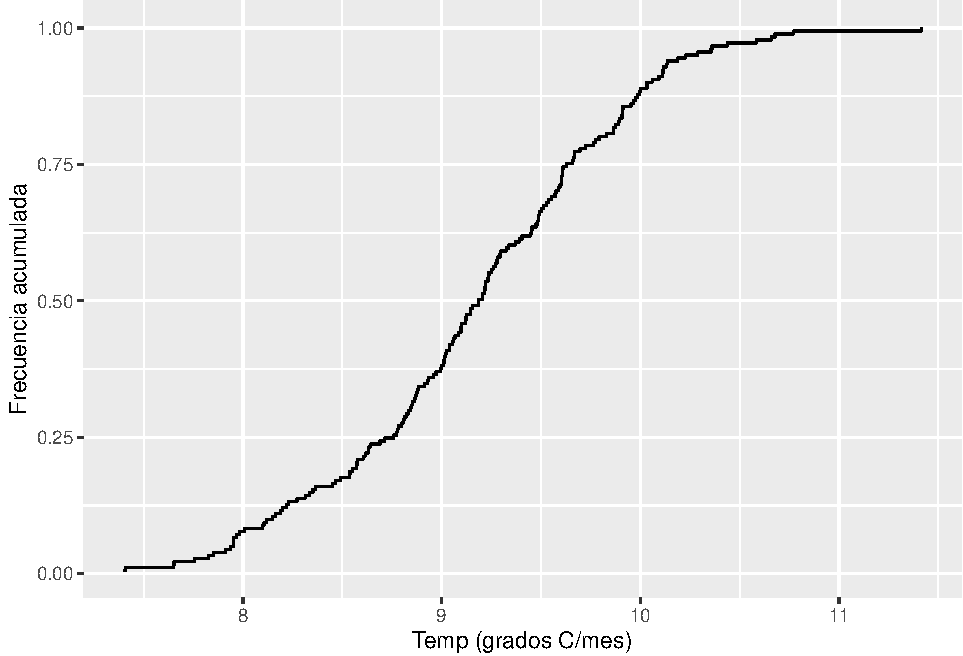
\includegraphics{Hidrology_files/figure-latex/unnamed-chunk-23-1.pdf}
\caption{Distribución empírica acumulada de temperatura}
\end{figure}

En la \textbf{Fig.12} se observa la distribución empírica acumulada de
la temperatura, es evidente notar que la probabilidad de encontrar
temperaturas menores a \(11^{\circ}C\) es alta, lo contrario pasa con
valores muy bajos del parámetro. Es poco probable encontrar valores
cercanos a cero; de hecho los valores más comunes se encuentran
alrededor del rango de \(8\) a \(11^{\circ}C\)

En la \textbf{Fig.13} se muestra el modelo de temperatura construido a
partir de los datos del sensor HOBO. Cabe la pena aclarar que éste es
una aproximación y no es un modelo que ajuste bien los datos. Es válido
decir esto dado la baja cantidad de puntos utilizados (\(8\)), son
pocos, pues se tomaron las coordenadas de los instrumentos instalados.
Se puede notar el gradiente mostrado en el mapa que sugiere la
variabilidad de la temperatura en el páramo; los rangos mostrados
difieren en aproximadamente \(3^{\circ}C\). Al observar este
comportamiento, se procedió a verificar si la altitud tenía influencia
sobre la temperatura; lo esperado sería que sí la tuviera
\cite{basantes}. Para determinar la relación se hace un test de
correlación arrojando un resultado de \(-0.46\) lo cual indica que
mientras una variable aumenta la otra disminuye, sin embargo, el mismo
valor en sí deja en duda si es una relación lineal, pues se encontró un
\(R^2\) de \(0.22\), lo que demuestra que si bien hay una conexión en
entre los parámetros ésta puede fluctuar y no ser constante, es decir,
pueden haber lugares altos pero con temperaturas más altas de lo normal;
éste comportamiento no sigue el descrito por \cite{van} que afirma que
la tasa de cambio, en promedio, de la temperatura con respecto a la
altitud, está típicamente entre \(-0.6\) y \(-0.7^{\circ}C\)
\(100 \ m-1\) ascendidos debido a la disminución de temperatura causada
por el desplazamiento de vientos cálidos desde zonas bajas que pierden
calor al elevarse, esto viene acompañado de otros efectos secundarios
\cite{buyta} los cuales no serán tratados acá.

\begin{figure}
\centering
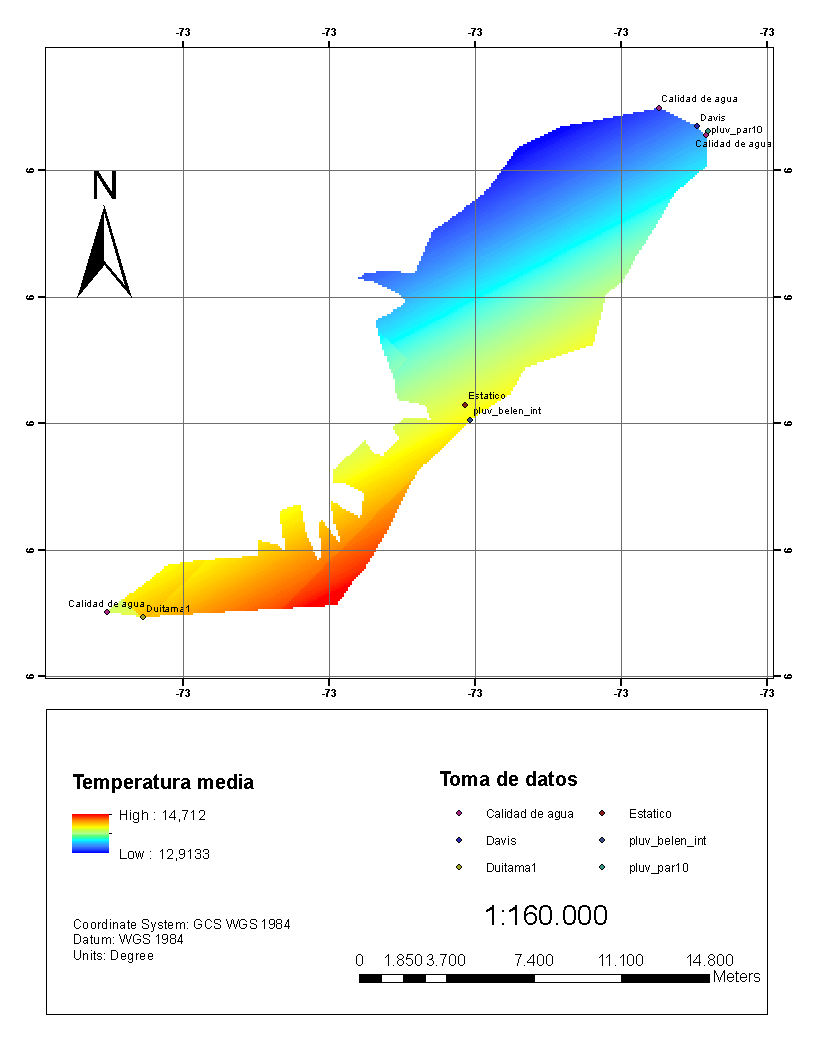
\includegraphics{paramo3.png}
\caption{Modelo de temperatura}
\end{figure}

\hypertarget{conclusiones}{%
\section{Conclusiones}\label{conclusiones}}

Las variables climáticas están íntimamente relacionadas, una depende la
otra como un ciclo que necesita de su entorno, las influencias pueden
variar de manera positiva o negativa, es decir, que si una aumenta la
otra disminuye o viceversa, es urgente entonces prestar atención a
fenómenos como el cambio climático que modifica algunas variables del
ambiente, esto repercute en el entorno alterando las fases naturales y
llevando consigo la disminución de la calidad de vida para todos los
seres vivos.

El clima en el páramo de La Rusia presenta la variabilidad esperada con
su temperatura máxima de \(19.5^{\circ}C\) a medio día y una mínima de
\(1.6^{\circ}C\) en la madrugada, una humedad relativa constantemente
alta a excepción del tiempo donde se tiene la temperatura más elevada,
haciendo de este un páramo muy húmedo, que si se tiene una buena
regeneración del ecosistema con unos suelos ricos en porosidad y óptimos
en infiltración, ayudado de la vegetación, puede ser muy importante para
la captura de agua y alimentación de los acuíferos subterráneos y ríos,
proporcionando así un buen rendimiento hídrico. Por lo tanto se hace
necesario estudios más detallados para el entendimiento y conservación
de estos ecosistemas, sobre todo en un país como Colombia que tiene la
mitad de páramos del mundo.

En los datos analizados es posible notar la alta variabilidad de la
precipitación en los Andes tropicales, el característico gradiente
altitudinal de la precipitación y la temperatura y la formación de
climas locales debidos a las barreras orográficas. Para tener una
comprensión holística de de esto es importante tener en cuenta y
estudiar a profundidad la relación suelo- atmósfera- vegetación del
clima tropical.

Se observó durante la práctica que el mayor impacto en estos páramos se
da por el uso indiscriminado que se le ha dado, principalmente ganadería
y agricultura lo que implica deforestación y degradación de suelos
afectando no sólo la disponibilidad de agua localmente sino también el
reciclaje de la precipitación.

Los páramos son ecosistemas muy sensibles no sólo por su papel
eco-hidrológico sino también por la dependencia antrópica de estas
fuentes para obtener agua de forma constante, a bajo costo y de calidad;
aspectos que se ven afectados cuando se intervienen en mayor o menor
grado. Por lo cual, es necesario realizar investigaciones sobre los
impactos antrópicos y la relación de estos impactos con el cambio en las
funciones en cuanto a rendimiento y regulación hídrica.

\end{document}


